\documentclass[a4paper]{article}

\usepackage{color}
\usepackage{url}
\usepackage[T2A]{fontenc} 
\usepackage[utf8]{inputenc}
\usepackage{graphicx}

\usepackage[english,serbian]{babel}
\usepackage[unicode]{hyperref}
\hypersetup{colorlinks,citecolor=red,filecolor=green,linkcolor=blue,urlcolor=blue}

\title{Slučajevi upotrebe Administratora sistema}


\begin{document}

\maketitle

\section{Slučajevi upotrebe}

\subsection{Administrator sistema}
\subsubsection{Slučaj upotrebe: Kreiranje naloga zaposlenom}
\begin{enumerate}
    \item \textbf{Kratak opis:} Administrator kreira nalog zaposlenoj osobi u kompaniji, čime je pomenutoj osobi omogućen pristup sistemu.
    \item \textbf{Učesnici:}
        \begin{itemize}
            \item Administrator
        \end{itemize}
    \item \textbf{Preduslovi:} Sistem je u funkciji. Administrator ima pristup internetu, sistemu, kao i privilegije potrebne za kreiranje naloga. Osnovne informacije o zaposlenom su validirane i prosleđene administratoru od strane menadžera ljudskih resursa.
    \item \textbf{Postuslovi:} Korisnički nalog za zaposlenog je uspešno kreiran. Baza zaposlenih je ažurirana.
    \item \textbf{Osnovni tok:}
        \begin{enumerate}
            \item Administrator otvara stranicu za kreiranje novog naloga.
            \item Sistem prikazuje stranicu sa listom obaveznih i opcionih polja koja jasno definišu nalog zaposlenog (ime, prezime, godište, pozicija itd...).
            \item Administrator popunjava sva obavezna polja.
            \item Administrator unosi jedinstveno korisničko ime / lozinku koje će zaposleni koristiti za budući pristup sistemu.
            \item Administrator potvrđuje unos.
        \end{enumerate}
    \item \textbf{Alternativni tokovi:}
        \begin{enumerate}
            \item \textbf{Administrator nije uneo sve obavezne informacije o zaposlenom.} Ukoliko administrator nije ispunio uslove koraka (c), sistem ga obaveštava o poljima koja su obavezna, a bez trenutne vrednosti i vraća na korak (b).
            \item \textbf{Administrator nije izabrao jedinstveno korisničko ime zaposlenog.} Ukoliko je administrator izabrao korisničko ime koje već pripada zaposlenom u firmi (Na primer, administrator definise korisničko ime po formatu ime.prezime, a u datom momentu dva zaposlena imaju identično ime i prezime), sistem ga obaveštava, nudi alternative koje prate već postojeći format i vraća na korak (d).
        \end{enumerate}
    \item \textbf{Podtokovi:} /
    \item \textbf{Specijalni zahtevi:}
        \begin{itemize}
            \item Lozinka mora biti kreirana sa kratkim vremenskim periodom validnosti (na primer 2 dana). Zaposleni mora biti obavešten o datom vremenskom periodu, i ručno promeniti lozinku nakon uspešnog prijavljivanja u sistem.
        \end{itemize}
    \item \textbf{Dodatne informacije:} Administrator ima pristup listi svih zaposlenih u kompaniji. Obavezne informacije za zaposlenog su: ime, prezime, datum rodjenja, pozicija, trenutna lokacija rada (grad/država).
\end{enumerate}

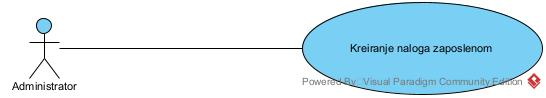
\includegraphics[scale=0.5]{SlucajUpotrebe_KreiranjeNalogaZaposlenom.jpg}

\subsubsection{Slučaj upotrebe: Deaktiviranje naloga osobama koje su prekinule radni odnos}
\begin{enumerate}
    \item \textbf{Kratak opis:} Administrator deaktivira nalog osobi koja prekida radni odnos u kompaniji, pomenuta osoba gubi mogućnost pristupa sistemu.
    \item \textbf{Učesnici:}
        \begin{itemize}
            \item Administrator
        \end{itemize}
    \item \textbf{Preduslovi:} Sistem je u funkciji. Administrator ima pristup internetu, sistemu, kao i privilegije potrebne za deaktiviranje naloga.
    \item \textbf{Postuslovi:} Korisnički nalog je deaktiviran. Korišćenjem korisničkog imena i lozinke nije moguće pristupiti sistemu
    \item \textbf{Osnovni tok:}
        \begin{enumerate}
            \item Administrator otvara stranicu sa listom svih zaposlenih u kompaniji.
            \item Sistem prikazuje listu svih zaposlenih i polje za pretragu zaposlenih po korisničkom imenu
            \item Administrator unosi korisničko ime zaposlenog u polje za pretragu.
            \item Sistem otvara stranicu zaposlenog sa svim pratećim podacima o istom.
            \item Administrator bira deaktivaciju naloga
            \item Sistem otvara stranicu potvrde o zatraženoj akciji uz upozorenje o posledicama operacije
            \item Administrator potvrđuje unos.
        \end{enumerate}
    \item \textbf{Alternativni tokovi:}
        \begin{enumerate}
            \item \textbf{Uneto korisničko ime ne odgovara nijednom zaposlenom.} Ukoliko pretraga zaposlenog po korisničkom imenu ne vrati rezultate, interfejs obaveštava administratora i vraća ga na korak (b).
        \end{enumerate}
    \item \textbf{Podtokovi:} /
    \item \textbf{Specijalni zahtevi:} /
    \item \textbf{Dodatne informacije:} Deaktivacija implicira odloženo brisanje naloga. Nakon deaktivacije nije moguće pristupiti datom nalogu, ali će sam nalog biti zadržan u bazi zaposlenih kroz kraći vremenski period radi lakšeg povraćaja naloga u ekstremnim situacijama (Na primer, u slučaju da je došlo do pogrešnog brisanja naloga). Nalog će biti permanentno obrisan kada pomenuti vremenski period istekne.
\end{enumerate}

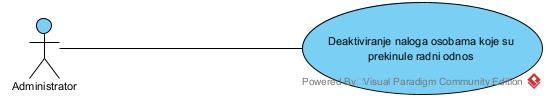
\includegraphics[scale=0.5]{SlucajUpotrebe_DeaktiviranjeNaloga.jpg}

\end{document}